% ===========================================================================
% Late-Interaction Retrieval of Regulatory DNA Sequences
% Progress Report — ICML 2-column style
%
% NOTE: This document uses a self-contained ICML-like format.
% If the icml2024.sty file is available, replace the preamble with:
%   \documentclass[accepted]{icml2024}
%   and use the standard ICML author macros.
% ===========================================================================

\documentclass[10pt,twocolumn]{article}

% ---------- Page geometry (ICML-like) ----------
\usepackage[letterpaper,margin=1in,columnsep=0.25in]{geometry}
\raggedbottom

% ---------- Fonts and typography ----------
\usepackage{times}
\usepackage[T1]{fontenc}
\usepackage[utf8]{inputenc}
\usepackage{microtype}

% ---------- Math ----------
\usepackage{amsmath,amssymb}

% ---------- Tables and figures ----------
\usepackage{booktabs}
\usepackage{graphicx}
\usepackage{multirow}
\usepackage{float}

% ---------- References and links ----------
\usepackage[colorlinks=true,citecolor=blue,linkcolor=blue,urlcolor=blue]{hyperref}
\usepackage{natbib}
\bibliographystyle{abbrvnat}

% ---------- Formatting ----------
\usepackage{enumitem}
\setlist{nosep,leftmargin=*}
\usepackage{xcolor}
\usepackage{caption}
\captionsetup{font=small,labelfont=bf}

% ---------- Title formatting (ICML-like) ----------
\usepackage{titlesec}
\titleformat{\section}{\large\bfseries}{\thesection}{1em}{}
\titleformat{\subsection}{\normalsize\bfseries}{\thesubsection}{0.75em}{}
\titlespacing*{\section}{0pt}{1.5ex plus 0.5ex minus .2ex}{1ex plus .2ex}
\titlespacing*{\subsection}{0pt}{1ex plus 0.3ex minus .2ex}{0.5ex plus .1ex}

% ---------- Abstract environment ----------
\renewenvironment{abstract}{%
  \centerline{\large\bfseries Abstract}%
  \vspace{0.5ex}%
  \begin{quote}\small
}{%
  \end{quote}%
  \vspace{1ex}%
}

\begin{document}

% ===========================================================================
% Title block
% ===========================================================================
\twocolumn[
\begin{center}
{\LARGE\bfseries Late-Interaction Retrieval of Regulatory DNA Sequences\\
Using ColBERT and DNABERT-2\par}
\vskip 1em
{\large Rohan Gumaste \quad Gabrielle Cohn \quad Vihan Lakshman\\[0.3em]
\normalsize Massachusetts Institute of Technology, Cambridge, MA, USA}
\vskip 1.5em

\begin{minipage}{0.9\textwidth}
\begin{abstract}
We investigate ColBERT-style late-interaction retrieval over the ENCODE SCREEN registry of human candidate cis-regulatory elements (cCREs), using DNABERT-2 as the backbone encoder. We benchmark 8 methods---from random baselines through gapped k-mer features to a pretrained DNA language model---on a retrieval task supervised by transcription factor (TF) ChIP-seq binding profiles. Pretrained DNABERT-2 achieves the best sequence-based MRR (0.0093), 25\% above classical k-mer baselines, but contrastive fine-tuning consistently overfits due to label sparsity in the TF binding matrix. We present a detailed dataset analysis diagnosing this failure and motivate a transition to the DeepSEA benchmark for the remainder of the project.
\end{abstract}
\end{minipage}
\vskip 1.5em
\end{center}
]

% ===========================================================================
\section{Introduction}
\label{sec:intro}
% ===========================================================================

The human genome contains approximately one million candidate cis-regulatory elements (cCREs)---promoters, enhancers, and insulators---cataloged by the ENCODE SCREEN registry~\citep{encode2020screen}. These regulatory switches control gene expression programs, yet determining functional similarity between elements remains an open problem. We ask: \emph{given only raw DNA sequence ($\sim$512 characters of ACGT), can we retrieve functionally similar regulatory elements?}

We apply ColBERT-style late-interaction retrieval~\citep{khattab2020colbert} with DNABERT-2~\citep{zhou2023dnabert2}, a 117M-parameter pretrained DNA language model using BPE tokenization. Late interaction is a natural fit for regulatory DNA because function arises from sparse combinations of transcription factor (TF) binding motifs (6--20\,bp) embedded in longer sequences (200--1000+\,bp). ColBERT's MaxSim scoring finds the best-matching position in the document for each query token, tolerating positional variation and rewarding partial motif overlap---properties that mean pooling into a single vector cannot express.

This progress report presents (1)~a comprehensive baseline evaluation on an ENCODE SCREEN retrieval benchmark with TF binding supervision, (2)~analysis of training dynamics showing consistent overfitting under contrastive fine-tuning, and (3)~a dataset-level diagnosis motivating a switch to the DeepSEA benchmark~\citep{zhou2015deepsea} for the remainder of the project.

% ===========================================================================
\section{Methods}
\label{sec:methods}
% ===========================================================================

\subsection{Dataset}
\label{sec:dataset}

We use cCREs from the ENCODE SCREEN V3 registry (GRCh38), which catalogs 1,063,878 human cCREs classified into 5 regulatory classes based on epigenomic signatures: PLS (promoter-like), pELS (proximal enhancer-like), dELS (distal enhancer-like), CTCF-only, and DNase-H3K4me3. We sample a 50k-element subset with chromosome-held-out splits: validation on chr2/chr10, test on chr1/chr8/chr21.

\textbf{Similarity signal.}
We define biological similarity via the integrated ENCODE TF ChIP-seq peaks matrix (ENCFF257UKO): a 2,818-dimensional binary vector per cCRE recording which TF experiments show a binding peak at that locus. Positive pairs require same regulatory class and TF overlap $\geq 2$; negatives are stratified by difficulty (cross-class, same-class with low overlap).

\subsection{Model}
\label{sec:model}

\textbf{Backbone.}
DNABERT-2 (117M parameters) uses BPE tokenization over DNA sequences, producing 768-dimensional hidden states across 12 transformer layers with 12 attention heads.

\textbf{ColBERT architecture.}
A shared DNABERT-2 encoder maps both query and document sequences to token-level representations. A learned linear projection reduces dimensionality from 768 to 64, followed by L2 normalization. Scoring follows the standard MaxSim formulation:
\begin{equation}
\text{score}(Q, D) = \sum_{i=1}^{m} \max_{j=1}^{n}\; q_i^\top d_j
\label{eq:maxsim}
\end{equation}
where $q_i, d_j \in \mathbb{R}^{64}$ are normalized token embeddings and the sum runs over non-padding query tokens.

\textbf{Fine-tuning.}
We apply LoRA (rank~16, $\alpha{=}32$, dropout~0.1) to $W_{qkv}$ and dense layers, reducing trainable parameters from 117M to ${\sim}2$M. Training uses multi-positive InfoNCE loss with temperature $\tau{=}0.1$:
\begin{equation}
\mathcal{L} = -\frac{1}{|B|} \sum_{i \in B} \log \frac{\sum_{j \in P_i} \exp(s_{ij}/\tau)}{\sum_{k=1}^{N} \exp(s_{ik}/\tau)}
\end{equation}
with gradient accumulation over 4~steps (effective batch size 80 queries) and DataParallel across $2{\times}$~RTX~2080~Ti.

\subsection{Baselines}
\label{sec:baselines}

We evaluate 8 baselines spanning nuisance checks, classical sequence methods, neural methods, and an oracle upper bound:

\begin{enumerate}
    \item \textbf{Random}: uniform random scores (absolute floor).
    \item \textbf{GC-matched random}: random within same GC-content decile (confound check).
    \item \textbf{K-mer cosine ($k{=}6$)}: 6-mer frequency vector cosine similarity (4,096 dimensions).
    \item \textbf{TF-IDF k-mer}: IDF-weighted 6-mer cosine; downweights common k-mers.
    \item \textbf{MinHash k-mer Jaccard}: approximate set Jaccard via 128 MinHash signatures.
    \item \textbf{Gapped k-mer (gkm-SVM style)}: gapped k-mers ($k{=}10$, $l{=}6$ informative positions) cosine; standard regulatory DNA baseline~\citep{ghandi2014gkmsvm}.
    \item \textbf{Pretrained DNABERT-2}: mean-pooled 768-dim embeddings, zero-shot, no fine-tuning.
    \item \textbf{Oracle}: cosine on true 2,818-dim TF binding vectors (upper bound; no sequence used).
\end{enumerate}

% ===========================================================================
\section{Experiments \& Results}
\label{sec:results}
% ===========================================================================

\subsection{Evaluation Setup}

We evaluate on 512 test queries against a corpus of 2,048 documents, all from chromosome-held-out test splits (chr1/chr8/chr21). Metrics include Mean Reciprocal Rank (MRR), normalized Discounted Cumulative Gain (nDCG), Recall@$k$ ($k \in \{1, 5, 10, 50\}$), top-$k$ cCRE class purity, and TF activity Jaccard@$k$.

\subsection{Baseline Results}

\begin{table*}[t]
\caption{Retrieval performance on the ENCODE SCREEN test set (512 queries, 2,048 corpus documents). Best sequence-based method in \textbf{bold}; oracle shown separately as an upper bound. All values are means across queries.}
\label{tab:baselines}
\vskip 0.5ex
\centering
\small
\begin{tabular}{@{}lccccccc@{}}
\toprule
\textbf{Baseline} & \textbf{MRR} & \textbf{nDCG} & \textbf{R@5} & \textbf{R@10} & \textbf{R@50} & \textbf{Purity@10} & \textbf{Act.Jac@10} \\
\midrule
Random              & 0.0054 & 0.0033 & 0.0010 & 0.0010 & 0.0073 & 0.687 & 0.006 \\
GC-matched          & 0.0055 & 0.0038 & 0.0005 & 0.0020 & 0.0088 & 0.590 & 0.008 \\
\addlinespace
K-mer cosine        & 0.0074 & 0.0056 & 0.0020 & 0.0034 & 0.0127 & 0.621 & 0.012 \\
TF-IDF k-mer        & 0.0062 & 0.0058 & 0.0015 & 0.0024 & 0.0146 & 0.624 & 0.012 \\
MinHash             & 0.0082 & 0.0050 & 0.0020 & 0.0024 & 0.0103 & 0.624 & 0.010 \\
gkm-SVM             & 0.0063 & 0.0058 & 0.0015 & 0.0024 & 0.0151 & 0.622 & 0.011 \\
\addlinespace
DNABERT-2 (pretrained) & \textbf{0.0093} & \textbf{0.0071} & \textbf{0.0024} & \textbf{0.0039} & \textbf{0.0161} & \textbf{0.645} & 0.011 \\
\midrule
Oracle (TF vectors) & 0.0317 & 0.0261 & 0.0073 & 0.0176 & 0.0562 & 0.637 & 0.167 \\
\bottomrule
\end{tabular}
\end{table*}

Table~\ref{tab:baselines} presents the full baseline comparison. Several findings emerge.

\textbf{No GC confound.}
GC-matched random performs indistinguishably from uniform random (MRR 0.0055 vs.\ 0.0054), confirming that retrieval signal is not driven by base composition.

\textbf{Pretrained DNABERT-2 is the best sequence method.}
Without any task-specific training, mean-pooled DNABERT-2 achieves MRR~0.0093---25\% above k-mer cosine (0.0074) and 14\% above MinHash (0.0082). Pretrained DNA language model representations capture regulatory patterns beyond what k-mer counting can express.

\textbf{Classical baselines cluster together.}
K-mer cosine (0.0074), TF-IDF (0.0062), MinHash (0.0082), and gkm-SVM (0.0063) all fall in the MRR 0.006--0.008 range. Notably, gkm-SVM---designed specifically for regulatory DNA~\citep{ghandi2014gkmsvm}---does not outperform simple 6-mer cosine, suggesting that gapped k-mer patterns add little signal for TF binding retrieval on this dataset.

\textbf{Oracle ceiling reveals headroom.}
The oracle achieves MRR 0.0317 ($3.4{\times}$ the best sequence method). Activity Jaccard@10 jumps from 0.011 to 0.167 ($15{\times}$). A perfect TF binding predictor would dramatically improve retrieval, but the gap also reflects the inherent lossiness of the sequence$\rightarrow$TF binding mapping.

\textbf{Low absolute numbers reflect label sparsity.}
Recall@50 below 2\% for all sequence methods is a consequence of the TF binding labels: most same-class cCRE pairs share zero TFs, making relevant items extremely sparse relative to corpus size.

\subsection{Training Dynamics}
\label{sec:training}

We attempted contrastive fine-tuning of the ColBERT model under four configurations (Table~\ref{tab:training}). All exhibit the same failure mode: the model memorizes training pairs without generalizing to held-out data.

\begin{table}[t]
\caption{Training configurations and outcomes. All runs use DNABERT-2 + LoRA + ColBERT. GA = gradient accumulation steps. Configs~A--B use 6-dim class proxy supervision; C--D use 2,818-dim TF vectors.}
\label{tab:training}
\vskip 0.5ex
\centering
\small
\begin{tabular}{@{}cccp{3.6cm}@{}}
\toprule
\textbf{Cfg} & $\boldsymbol{\tau}$ & \textbf{GA} & \textbf{Result} \\
\midrule
A & 0.05 & 1 & Loss stagnates at random baseline after epoch~1 \\
\addlinespace
B & 0.1  & 1 & Train loss~$\downarrow$, val MRR flat at 0.051 over 10~epochs \\
\addlinespace
C & 0.1  & 1 & Same stagnation; epoch~2 flattens at loss~4.88 \\
\addlinespace
D & 0.1  & 4 & Train loss~$\rightarrow$~1.68, val loss stays~4.90 (overfit) \\
\bottomrule
\end{tabular}
\end{table}

Gradient accumulation (Config~D) was the only setting that broke below the random-loss baseline during training, achieving a train loss of 1.68 versus the random baseline of ${\sim}4.9$. However, the validation loss remained at 4.90---a train/val gap of 3.2~nats---indicating pure memorization. Neither richer supervision (6-dim~$\rightarrow$~2,818-dim) nor temperature tuning resolved the generalization failure. This consistent pattern points to a \emph{dataset-level} limitation rather than a model or optimization deficiency, motivating the analysis in Section~\ref{sec:analysis}.

% ===========================================================================
\section{Dataset Analysis}
\label{sec:analysis}
% ===========================================================================

The training failures motivated a thorough exploratory analysis of the TF binding supervision signal, which reveals fundamental limitations of the current dataset for contrastive learning.

\subsection{TF Binding Vector Properties}

\textbf{Sparsity.}
Of the 50k cCREs in our subset, 20.6\% (10,301 elements) have zero TF binding peaks and cannot participate meaningfully in TF-supervised training. The median number of TFs per cCRE is only 7 out of 2,818 experiments (Figure~\ref{fig:tf_density}).

\begin{figure}[t]
\centering
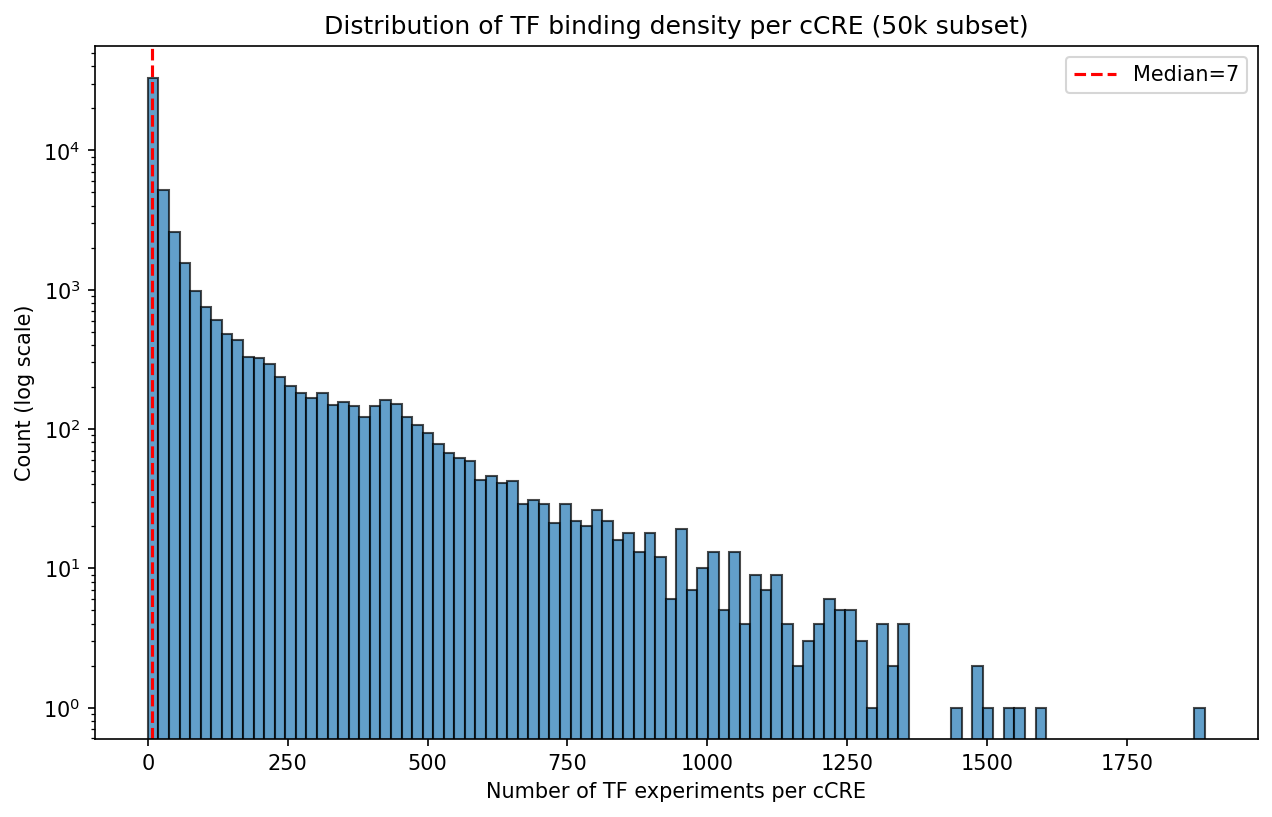
\includegraphics[width=\columnwidth]{figures/task1_ccre_tf_density.png}
\caption{Distribution of TF binding experiments per cCRE. The distribution is heavily right-skewed with median~7 and 20.6\% of cCREs at zero.}
\label{fig:tf_density}
\end{figure}

\textbf{Pairwise similarity is near-zero.}
Same-class Jaccard similarity has median~0.000, mean~0.038, and 95th percentile~0.213 (Figure~\ref{fig:jaccard}). Most same-class pairs share effectively no TF binding---the supervision signal is concentrated in a small fraction of pairs.

\begin{figure}[t]
\centering
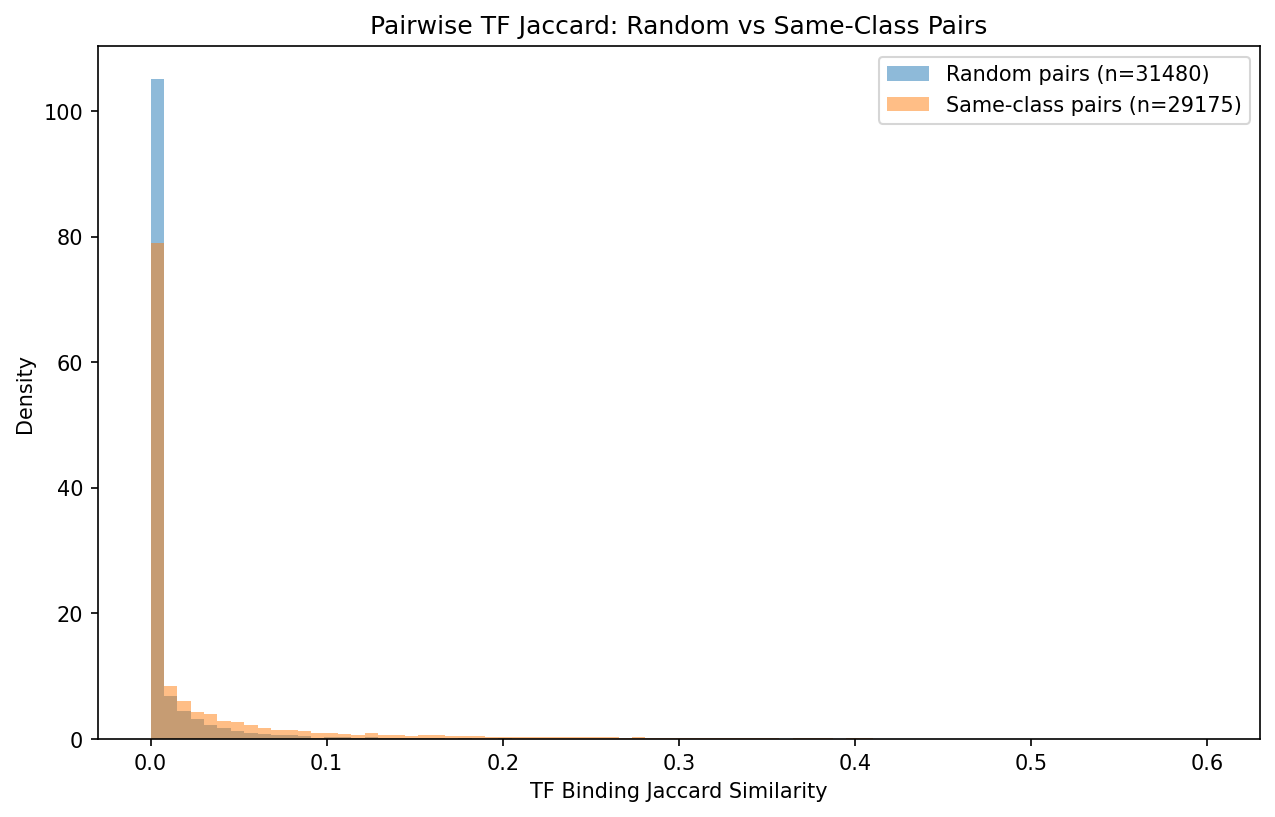
\includegraphics[width=\columnwidth]{figures/task1_jaccard_distributions.png}
\caption{Pairwise Jaccard distributions for random pairs and same-class pairs. Both are heavily concentrated at zero.}
\label{fig:jaccard}
\end{figure}

\textbf{Threshold dilemma.}
No positive-pair threshold cleanly separates meaningful similarity from noise:
\begin{itemize}
    \item Jaccard $\geq 0.5$ leaves 89\% of queries with zero positives (too strict).
    \item Overlap $\geq 2$ yields positives dominated by housekeeping TFs: CTCF (28\%) and POLR2A (35\%) (too noisy).
\end{itemize}

\textbf{Weak sequence--function correlation.}
Pearson $r = 0.21$ between 6-mer cosine similarity and TF Jaccard (Figure~\ref{fig:kmer_vs_jaccard}). High-TF-Jaccard pairs have slightly higher k-mer similarity (0.159 vs.\ 0.136), confirming a real but subtle sequence signal.

\begin{figure}[t]
\centering
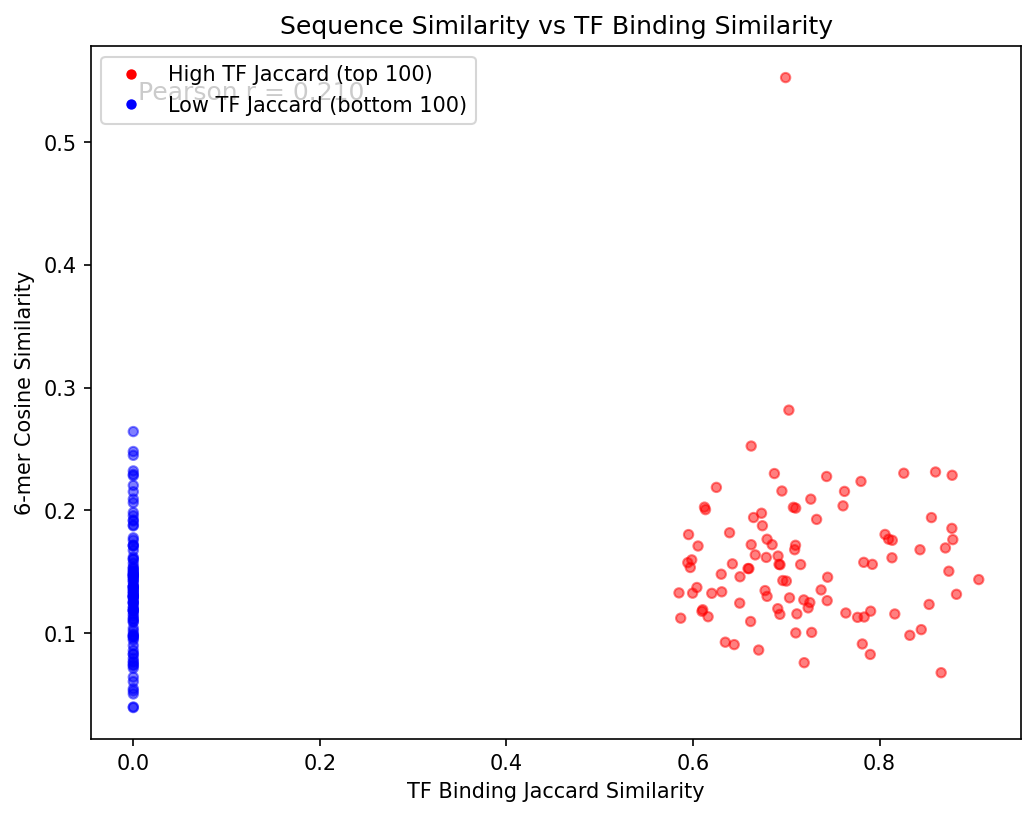
\includegraphics[width=\columnwidth]{figures/task4_kmer_vs_jaccard.png}
\caption{6-mer cosine similarity vs.\ TF Jaccard for high- and low-similarity same-class pairs (requiring $\geq$5 TFs each). Pearson $r = 0.21$.}
\label{fig:kmer_vs_jaccard}
\end{figure}

\subsection{Why the Current Dataset Limits Learning}

The TF binding matrix is sparse due to \emph{experimental coverage}, not biology: low Jaccard between two enhancers may indicate genuinely different function or simply that they were assayed in different cell lines. This introduces systematic label noise that contrastive learning amplifies. False negatives (truly similar elements scored as dissimilar due to missing assays) suppress gradient signal, while false positives (elements sharing only housekeeping TFs) inject noise.

The within-class substructure visible in t-SNE projections of TF binding vectors (Figure~\ref{fig:tsne}) confirms that real regulatory programs exist in the data. dELS elements form multiple distinct clusters corresponding to different regulatory programs. The problem is not absence of biological signal but our inability to extract clean supervision from the sparse, heterogeneous TF binding matrix.

\begin{figure}[t]
\centering
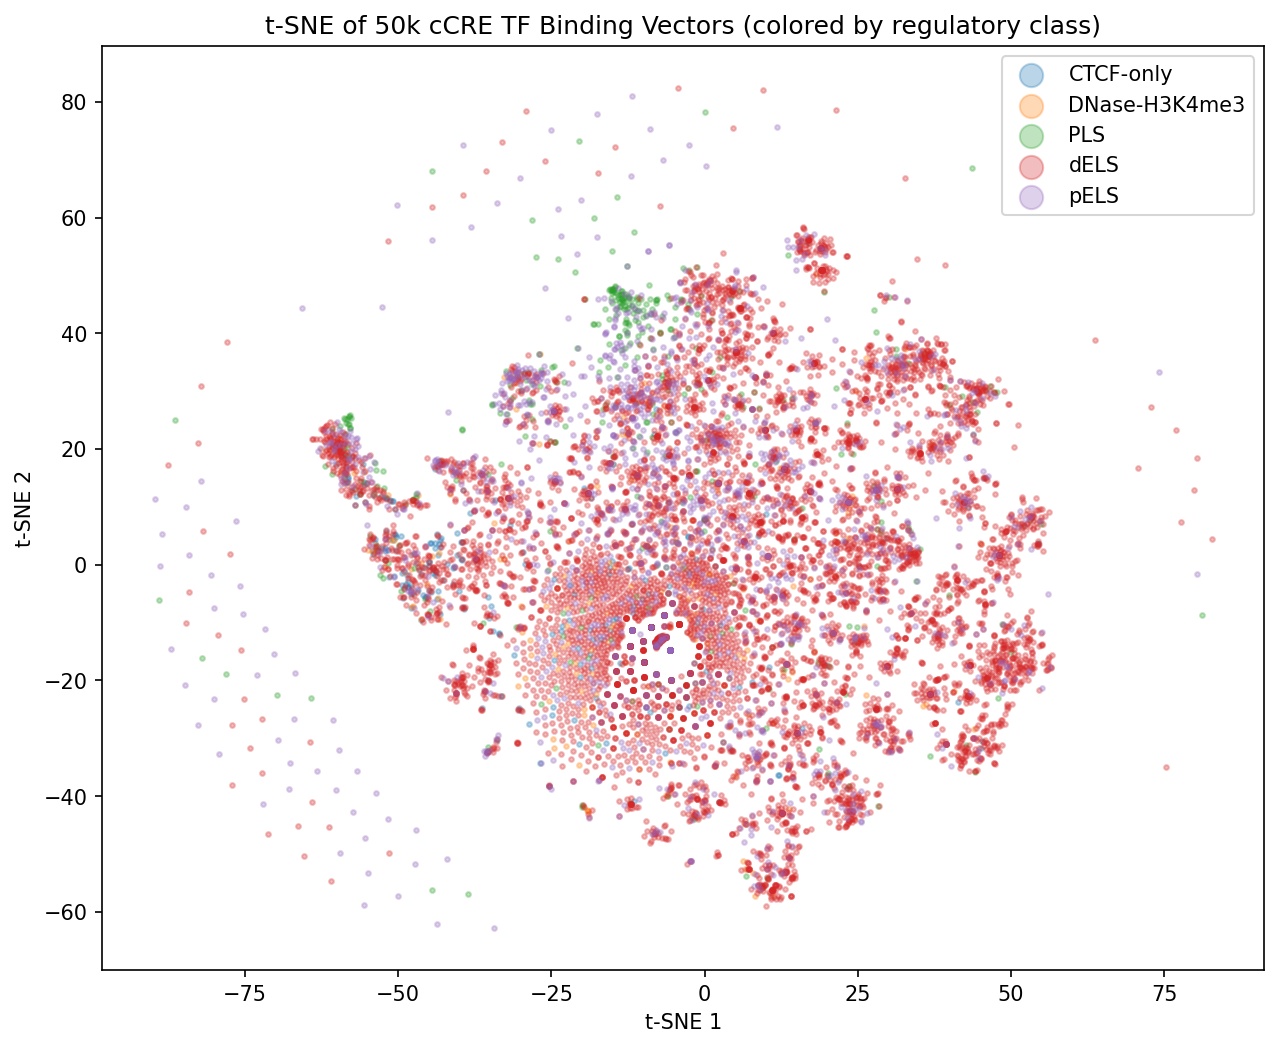
\includegraphics[width=\columnwidth]{figures/task5_t-sne_by_class.png}
\caption{t-SNE of TF binding vectors colored by regulatory class (10k subsample). dELS exhibits clear internal substructure with multiple distinct clusters corresponding to different regulatory programs.}
\label{fig:tsne}
\end{figure}

\subsection{Planned Switch to DeepSEA}
\label{sec:deepsea}

The DeepSEA dataset~\citep{zhou2015deepsea} provides a substantially cleaner supervision signal for contrastive retrieval:

\begin{itemize}
    \item \textbf{919 binary chromatin features} per 1kb sequence, spanning TF binding, DNase hypersensitivity, and histone marks across cell types.
    \item \textbf{Uniform genome-wide assays}: labels derived from standardized ChIP-seq and DNase-seq pipelines rather than heterogeneous experiment-specific peak calls.
    \item \textbf{Dense labels}: every sequence has annotations across all 919 features, eliminating the 20.6\%-zero-vector problem that plagues the ENCODE TF matrix.
    \item \textbf{Established benchmark}: known baselines and published results enable direct comparison.
\end{itemize}

Similarity under DeepSEA becomes cosine over a 919-dim dense vector---a much stronger training signal than Jaccard over 2,818 sparse binary dimensions. We expect this to resolve the contrastive training failures by providing cleaner positives and harder, more informative negatives.

% ===========================================================================
\section{Next Steps}
\label{sec:next}
% ===========================================================================

\textbf{Complete single-vector fine-tuned baseline.}
A mean-pooled DNABERT-2 model with identical LoRA fine-tuning and training pairs is currently in progress. This is the critical architectural comparison: if ColBERT's token-level MaxSim scoring does not improve over single-vector cosine, the late-interaction hypothesis for regulatory DNA is unsupported.

\textbf{Switch to DeepSEA.}
Redefine the retrieval task over DeepSEA's 919-dim chromatin feature vectors. Build positive/negative pairs from cosine similarity thresholds on the dense label space, where the threshold dilemma is substantially less severe.

\textbf{Regulatory program discovery.}
Apply NMF or $k$-means clustering on the chromatin feature matrix to discover latent regulatory programs (e.g., erythroid, neural). Reframe retrieval as ``same program'' membership prediction, yielding cleaner supervision and biologically interpretable evaluation.

\textbf{ColBERT vs.\ mean-pool on DeepSEA.}
With a dataset that supports successful contrastive training, directly compare late-interaction (MaxSim) against single-vector (mean-pool cosine) scoring on the same backbone and training configuration.

\textbf{Scale to full corpus.}
Expand from 50k to the full 1M+ cCRE corpus with FAISS-based approximate nearest neighbor indexing for efficient retrieval at scale.

% ===========================================================================
% References
% ===========================================================================

\small
\begin{thebibliography}{5}
\setlength{\itemsep}{2pt}
\setlength{\parsep}{0pt}

\bibitem[{ENCODE Project Consortium}(2020)]{encode2020screen}
ENCODE Project Consortium.
\newblock Expanded encyclopaedias of {DNA} elements in the human and mouse genomes.
\newblock \emph{Nature}, 583(7818):699--710, 2020.

\bibitem[Ghandi et~al.(2014)Ghandi, Lee, Mohammad-Noori, and Beer]{ghandi2014gkmsvm}
Ghandi, M., Lee, D., Mohammad-Noori, M., and Beer, M.~A.
\newblock Enhanced regulatory sequence prediction using gapped $k$-mer features.
\newblock \emph{PLoS Computational Biology}, 10(7):e1003711, 2014.

\bibitem[Khattab and Zaharia(2020)]{khattab2020colbert}
Khattab, O. and Zaharia, M.
\newblock {ColBERT}: Efficient and effective passage search via contextualized late interaction over {BERT}.
\newblock In \emph{Proceedings of the 43rd International ACM SIGIR Conference on Research and Development in Information Retrieval}, pp.\ 39--48, 2020.

\bibitem[Zhou and Troyanskaya(2015)]{zhou2015deepsea}
Zhou, J. and Troyanskaya, O.~G.
\newblock Predicting effects of noncoding variants with deep learning--based sequence model.
\newblock \emph{Nature Methods}, 12(10):931--934, 2015.

\bibitem[Zhou et~al.(2023)Zhou, Ji, Li, Dutta, Davuluri, and Liu]{zhou2023dnabert2}
Zhou, Z., Ji, Y., Li, W., Dutta, P., Davuluri, R.~V., and Liu, H.
\newblock {DNABERT-2}: Efficient foundation model and benchmark for multi-species genome.
\newblock \emph{arXiv preprint arXiv:2306.15006}, 2023.

\end{thebibliography}

\end{document}
